%for a more compact document, add the option openany to avoid
%starting all chapters on odd numbered pages
\documentclass[12pt]{cmuthesis}

% This is a template for a CMU thesis.  It is 18 pages without any content :-)
% The source for this is pulled from a variety of sources and people.
% Here's a partial list of people who may or may have not contributed:
%
%        bnoble   = Brian Noble
%        caruana  = Rich Caruana
%        colohan  = Chris Colohan
%        jab      = Justin Boyan
%        josullvn = Joseph O'Sullivan
%        jrs      = Jonathan Shewchuk
%        kosak    = Corey Kosak
%        mjz      = Matt Zekauskas (mattz@cs)
%        pdinda   = Peter Dinda
%        pfr      = Patrick Riley
%        dkoes = David Koes (me)

% My main contribution is putting everything into a single class files and small
% template since I prefer this to some complicated sprawling directory tree with
% makefiles.

% some useful packages
\usepackage{times}
\usepackage{fullpage}
\usepackage{graphicx}
\usepackage{amsmath}
\usepackage[numbers,sort]{natbib}
\usepackage{tabularx}
\usepackage{array}
\usepackage[table]{xcolor}
\usepackage{textcomp}
\usepackage{csquotes}
\usepackage[backref,pageanchor=true,plainpages=false, pdfpagelabels, bookmarks,bookmarksnumbered,
%pdfborder=0 0 0,  %removes outlines around hyper links in online display
]{hyperref}
\usepackage{subfig}

% Approximately 1" margins, more space on binding side
%\usepackage[letterpaper,twoside,vscale=.8,hscale=.75,nomarginpar]{geometry}
%for general printing (not binding)
\usepackage[letterpaper,twoside,vscale=.8,hscale=.75,nomarginpar,hmarginratio=1:1]{geometry}

% Provides a draft mark at the top of the document. 
\draftstamp{\today}{DRAFT}

\begin {document} 
\frontmatter

%initialize page style, so contents come out right (see bot) -mjz
\pagestyle{empty}

\title{ %% {\it \huge Thesis Proposal}\\
{\bf Title Pending}}
\author{Mihir Bala}
\date{XX 2025}
\Year{2025}
\trnumber{}

\committee{
Mahadev Satyanarayanan, Chair \\
David O'Hallaron \\
Jeff Schneider \\
Padmanabhan Pillai
}

\support{}
\disclaimer{}

% copyright notice generated automatically from Year and author.
% permission added if \permission{} given.

\keywords{Autonomous Drones, Robotics, Mobile Computing, Edge Computing}

\maketitle

\begin{dedication}
TBD
\end{dedication}

\pagestyle{plain} % for toc, was empty

%% Obviously, it's probably a good idea to break the various sections of your thesis
%% into different files and input them into this file...

\begin{abstract}
To be written.
\end{abstract}

\begin{acknowledgments}
To be written.
\end{acknowledgments}



\tableofcontents
\listoffigures
\listoftables

\mainmatter

%% Double space document for easy review:
%\renewcommand{\baselinestretch}{1.66}\normalsize

% The other requirements Catherine has:
%
%  - avoid large margins.  She wants the thesis to use fewer pages, 
%    especially if it requires colour printing.
%
%  - The thesis should be formatted for double-sided printing.  This
%    means that all chapters, acknowledgements, table of contents, etc.
%    should start on odd numbered (right facing) pages.
%
%  - You need to use the department standard tech report title page.  I
%    have tried to ensure that the title page here conforms to this
%    standard.
%
%  - Use a nice serif font, such as Times Roman.  Sans serif looks bad.
%
% Other than that, just make it look good...

\chapter{Introduction}
\label{sec:introduction}
Unmanned aerial vehicles, commonly known as drones, are a disruptive technology that have recently seen widespread use. In civilian settings, they enable cheap and safe completion of tasks such as infrastructure inspection, agriculture monitoring, wildfire control, and police surveillance. In military settings, they are a vital tool for advance reconnaissance. For most use cases today, drones are deployed with a human pilot who is in constant control of the aircraft.

In recent years, research efforts have pushed towards drones capable of fully-autonomous flight. The term \textit{fully-autonomous} flight is defined by the National Institute of Science and Technology (NIST) as “pre-programmed flight without a remote human pilot, including mission-specific actions in response to runtime observations”~\cite{Huang2008}. There are two main benefits to this approach. First, it decreases costs and frees human attention. Second, it allows the practical operation of drone swarms, large groups of aircraft that cooperatively execute tasks. Drone swarms open the door to many missions that could revolutionize several civilian and military sectors~\cite{Burkle2009}. 

A key driver for fully-autonomous drones is the completion of active vision tasks~\cite{Aloimonos1988, Ognibene2013}. Active vision tasks require a drone to react in real time to its current scene interpretation. For instance, it may drop down to lower altitude without human intervention ``to take a closer look'' before the scene changes.  It may then return to its original altitude to continue monitoring the scene. This narrow scope of tasks characterizes many fundamental drone operations like following a target and evading obstacles.

Weight is a fundamental impediment to fully-autonomous drone adoption. Greater intelligence correlates with more powerful (and hence heavier) on-board computing and richer sensing. An on-board GPU, for example, brings with it a long logistical tail: heatsinks, cooling fans, and larger batteries. Increased weight brings with it regulatory challenges for flights over civilian areas. Since 2021, the FAA has pre-authorized flights over people and vehicles by drones with a total weight of less than 250~g~\cite{FAA2021}. Heavier drones require explicit FAA approval for such flights, conditional upon mitigation measures for collisions and free fall. Even above this limit, regulatory approval for autonomous BVLOS (beyond visual line of sight) flight in dense urban settings is easier to obtain for lighter drones than for heavier drones. This regulation has proven to be a major obstacle for several civilian projects. In military settings, weight is also a crucial consideration. Heavy aircraft complicate logistics and often require dedicated transportation~\cite{DefensePost}. 

Other major limitations to autonomous drone adoption are software portability, accessibility, mission versatility, and unit cost. While there have been attempts to bring all drones under a unified programming ecosystem, it is still the norm for drone companies to develop their own SDKs for their platforms. This makes it difficult to port code written for one ecosystem to another which divides the development community. Existing fully-autonomous drones also require users to have significant flight experience to ensure safe operation, a serious barrier to accessibility. Many lack versatility, and cannot be configured to perform missions outside of a small, manufacturer specified set. Lastly, the unit cost for current autonomous drones is several times higher than manually piloted equivalents. Such prices hurt the economic viability of swarm operations where individual aircraft losses are not only likely but expected.

The core contribution of this work is \textit{SteelEagle}, a hardware-agnostic autonomous drone system which attempts to surmount these obstacles by leveraging edge computing and a new modular drone operating system. Edge computing enables a drone to offload compute-intensive real-time operations over a low-latency, high-bandwidth wireless network to a powerful ground-based server (cloudlet) which is usually located near a cell tower. This reduces the need for heavy on-board computing hardware. In parallel, the SteelEagle operating system is designed to be drone agnostic, developer friendly, and mission centric.

A key consideration of this system is the use of commercial off-the-shelf~\cite{FAR} (COTS) drones and computing / communication payloads. This approach avoids customization of hardware (e.g., drone modifications) and modification of privileged software (e.g., “rooting” a device) which lowers cost and greatly increases accessibility. It also avoids the need for re-certification (e.g., by the FAA or the FCC). However, a COTS approach also introduces new obstacles. Thermal limitations of lightweight COTS communications devices pose latency, frame rate, and quality challenges, and force such systems to intelligently manage communication, computation, and prediction.

\section{Thesis Statement}
In this dissertation, I demonstrate SteelEagle as a capable alternative to existing autonomous drone systems, despite the inherent latency and bandwidth limitations of offloading. I show how it improves over other platforms in the following design categories:

\begin{enumerate}
\item \textbf{Weight}: the overall weight of the aircraft, including batteries and payload.
\item \textbf{Accessibility}: the barrier-for-entry to operate the aircraft. 
\item \textbf{Versatility}: the diversity of tasks which the system can execute.
\item \textbf{Portability}: the ease with which the system can be ported to new hardware.
\item \textbf{Cost}: the overall cost of the aircraft, including batteries and payload.
\end{enumerate}
\\
In particular, I claim that:
\newpage
\textbf{It is feasible to construct an ultra-light flight platform for autonomous active vision tasks in beyond visual line-of-sight (BVLOS) settings that only uses commercial off-the-shelf (COTS) drones and COTS computing/communication payloads. The most serious obstacle to this goal, namely the weight of computing hardware necessary to achieve autonomy, can be overcome using edge computing. I posit that such a flight platform can emulate the performance of heavier autonomous drones on active vision tasks, despite bandwidth, latency and connectivity challenges.}

\textit{Why is this thesis important?} If this statement were true, then such edge-enabled drones could see widespread adoption for BVLOS missions in urban environments. They would have lower operation costs and increased safety compared to traditional autonomous drones. Tasks such as structure inspection, police surveillance, and traffic monitoring could directly benefit from this. Drone swarms over public infrastructure would become safer.

\textit{Why does it not follow trivially from what is already known?} Existing work in this space is limited since most current research focuses on improving drone capabilities rather than decreasing their weight. There are no commercial drones under the FAA threshold of 250~g that possess onboard intelligence capable of autonomously executing  missions. There are limited drones that are edge-enabled, but these drones are heavy (more than 500~g) and expensive (over \$3,000). There has been some academic research on using drones in conjunction with edge computing, with full details provided in Section~\ref{sec:drone-and-the-edge}. However, these efforts focused on large, heavy drones which used onboard hardware in addition to supplemental edge offload. None identified weight as a dominant design consideration. SteelEagle, by contrast, is designed primarily around reducing weight without compromising capability. It is my belief that this is critical to drive large scale adoption of autonomous drones. 

\begin{flushleft}
The main contributions of this thesis are as follows:
\end{flushleft}
\begin{enumerate}
\item I describe a fully-autonomous flight platform capable of executing active vision tasks on lightweight COTS drones using edge computing. I show why this platform is an improvement over prior work in terms of its \textit{weight}, \textit{accessibility}, \textit{versatility}, \textit{portability}, and \textit{cost}.
\item I provide a measurement study quantifying this platform's performance using a novel benchmarking suite.
\item I show how this platform can be extended to a heterogeneous drone swarm ecosystem.  
\end{enumerate}

 

\section{Thesis Overview}
The remainder of this dissertation is organized as follows:
\begin{itemize}
    \item In Chapter 2, I provide background on the development history of autonomous drones and summarize related research in this area. I show how SteelEagle builds on this existing research.
    \item In Chapter 3, I discuss how to connect lightweight COTS drones to the edge. I outline the design challenges and formulate a criteria for choosing an edge communication payload that flies with the drone.
    \item In Chapter 4, I provide the overall design of SteelEagle including its advantages and disadvantages over current systems. I demonstrate a SteelEagle drone performing several autonomous tasks and provide some performance analysis.
    \item In Chapter 5, I introduce a new edge communication payload that improves on the earlier prototype. I show how this new payload can reduce the OODA (Observe Orient Decide Act) loop of the system, and thus greatly increase autonomous performance.
    \item In Chapter 6, I describe a family of benchmarks for measuring edge-based and fully-onboard autonomous drone performance on several key tasks. These benchmarks stress the OODA loop of the given test platform and are useful for understanding the impact of high latency and low throughput on edge offloading.
    \item In Chapter 7, I deploy SteelEagle on new drone hardware to demonstrate drone hardware agnosticism. I illustrate how my system adapts to different hardware and how it can cope with disconnected operation.
    \item Finally, in Chapter 8, I conclude the dissertation and explain future work with a summary of contributions.
\end{itemize}


\chapter{Background and Related Work}
Autonomous drones are an emerging field in both civilian and military sectors. The investment in Zipline, DJI, and other similar companies, show that there is a lucrative market for urban autonomous drone applications such as same-day drone delivery, automated infrastructure inspection, and programmable aerial surveillance~\cite{GrandviewResearchDroneMarket,ForbesZiplineEvaluation}. The rise of companies like Anduril and recent geopolitical events like the War in Ukraine also hint at the wider role that autonomous drones will play in future armed conflicts~\cite{CNBC,CFAS}.

Even with this demand, the quest to make smaller, lightweight autonomous drones is ongoing. Weight scales closely with the capability of onboard compute, and artificial intelligence algorithms used for drone perception continue to require more computation to run. This makes the prospect of creating a drone system with real-time access to such algorithms challenging.

In this chapter, I provide background on current autonomous drone platforms and outline how some of the obstacles impeding their practical deployment can be overcome. In Section \ref{sec:history-drone-development}, I briefly describe the history of drone development and regulation along with the different categories of modern drones. I also explain the various problems holding these systems back from widespread adoption. In Section \ref{sec:prior-work}, I discuss prior research that has attempted to solve these problems, and its limitations. In Section \ref{sec:better-autonomous-drones}, I propose a possible solution by leveraging the benefits of edge computing and COTS hardware. I show how the advantages of this approach could make autonomous drone deployment in urban environments a reality.

\section{The Development of Modern Drones}
\label{sec:history-drone-development}

Research into drone technology started in the early 1900s when during the interwar period, British engineers created a radio controlled plane, nicknamed the ``Queen Bee'', to train their anti-aircraft gunnery~\cite{IWMDrone}. The Queen Bee's name would spawn the colloquial ``drone'' moniker when referring to radio-controlled aircraft, a reference to worker drones in bee colonies. Over the next several decades, militaries around the world began incorporating drones into their arsenals; first, as pilotless training targets but later, as remotely operated observation and strike aircraft. By the 1990s, drones had become very sophisticated, equipped with multiple onboard sensors which enabled these platforms to conduct aerial reconnaissance at great distances~\cite{GlobalHawk}. However, despite these advances, one core design tenet remained unchanged: drones were always controlled by a human pilot and had limited ability to function on their own.

\begin{figure}%
    \centering
    \subfloat[\centering The British-made "Queen Bee", introduced in 1935, was one of the first radio operated aircraft and served as an anti-aircraft practice target~\cite{IWMDrone}.]{{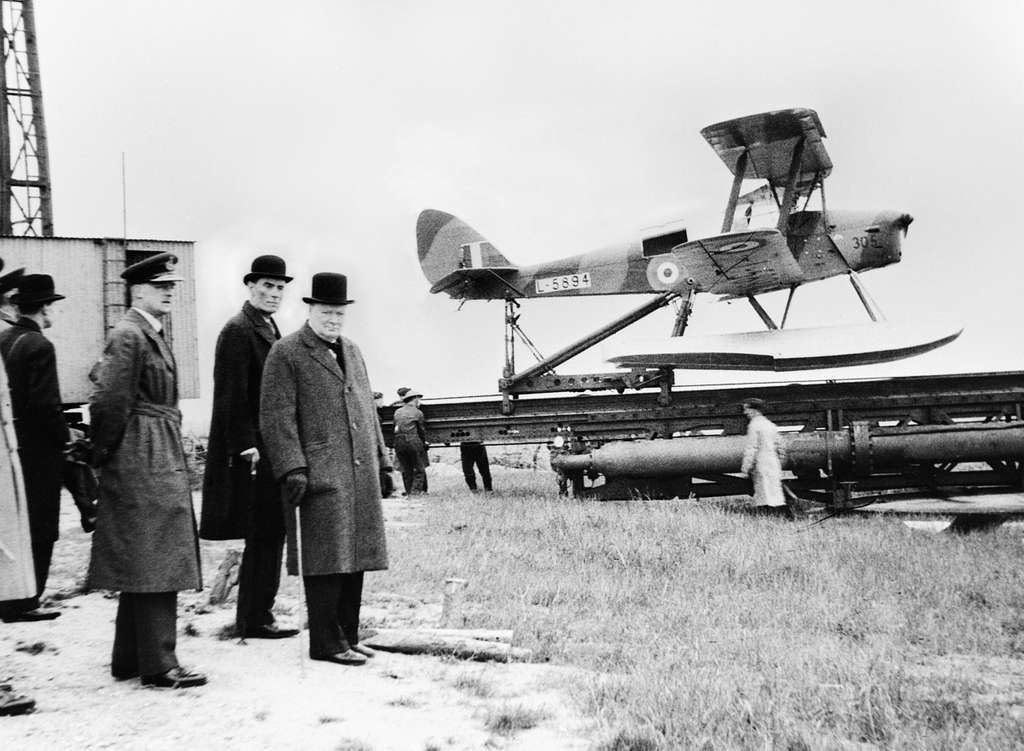
\includegraphics[width=7cm, height=5cm]{chapter2/FIGS/qbee2.jpg}}}%
    \qquad
\subfloat[\centering The RQ-4 Global Hawk, introduced in 1998, is a currently operated US Air Force reconnaissance drone with a range of over 14,000 miles~\cite{GlobalHawk}.]{{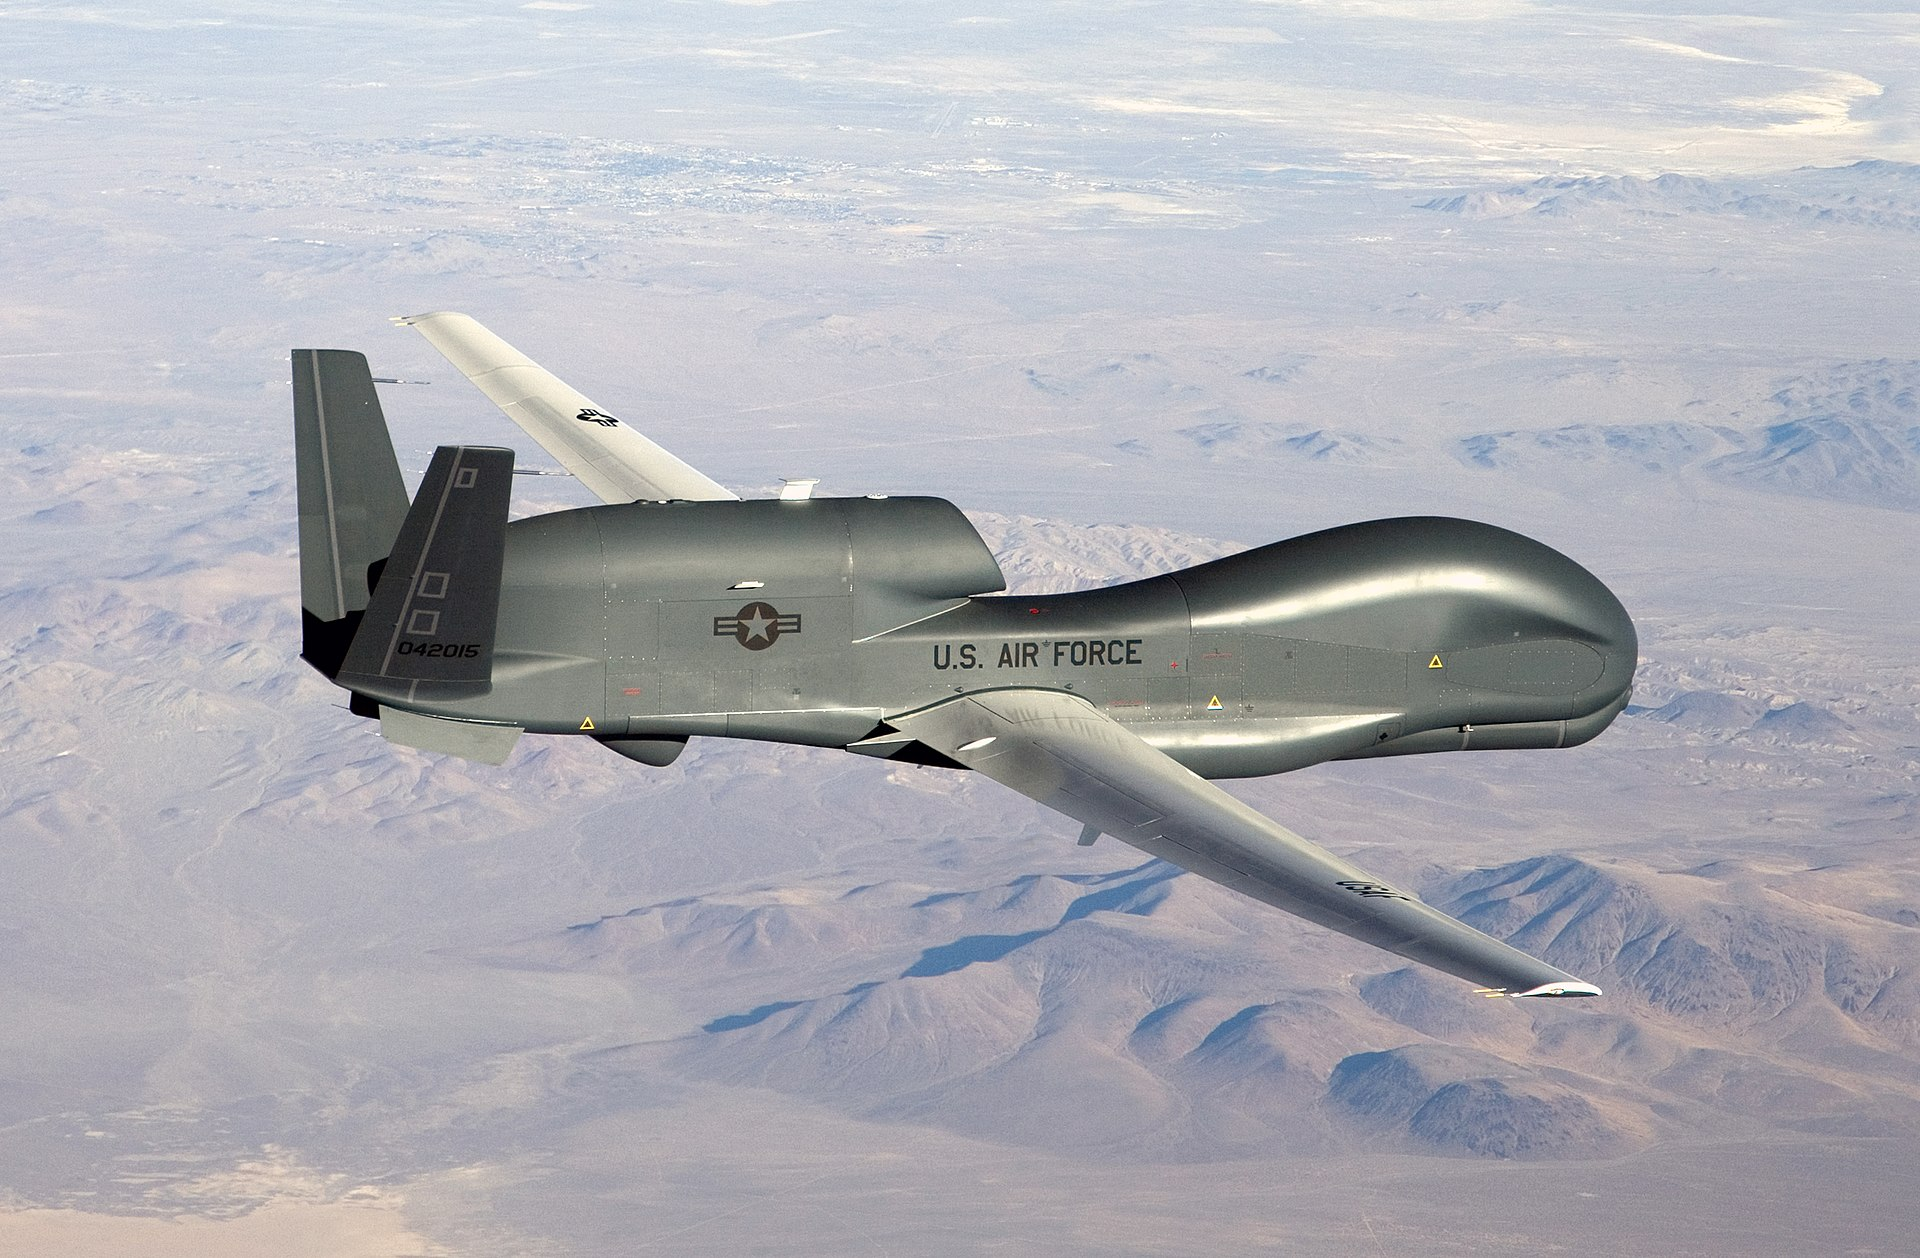
\includegraphics[width=7cm, height=5cm]{chapter2/FIGS/globalhawkdrone.jpg} }}%

    \subfloat[\centering The Skydio 2, released in 2019, provides a small set of semi- and fully-autonomous capabilities like person tracking and obstacle avoidance~\cite{Skydio2}.]{{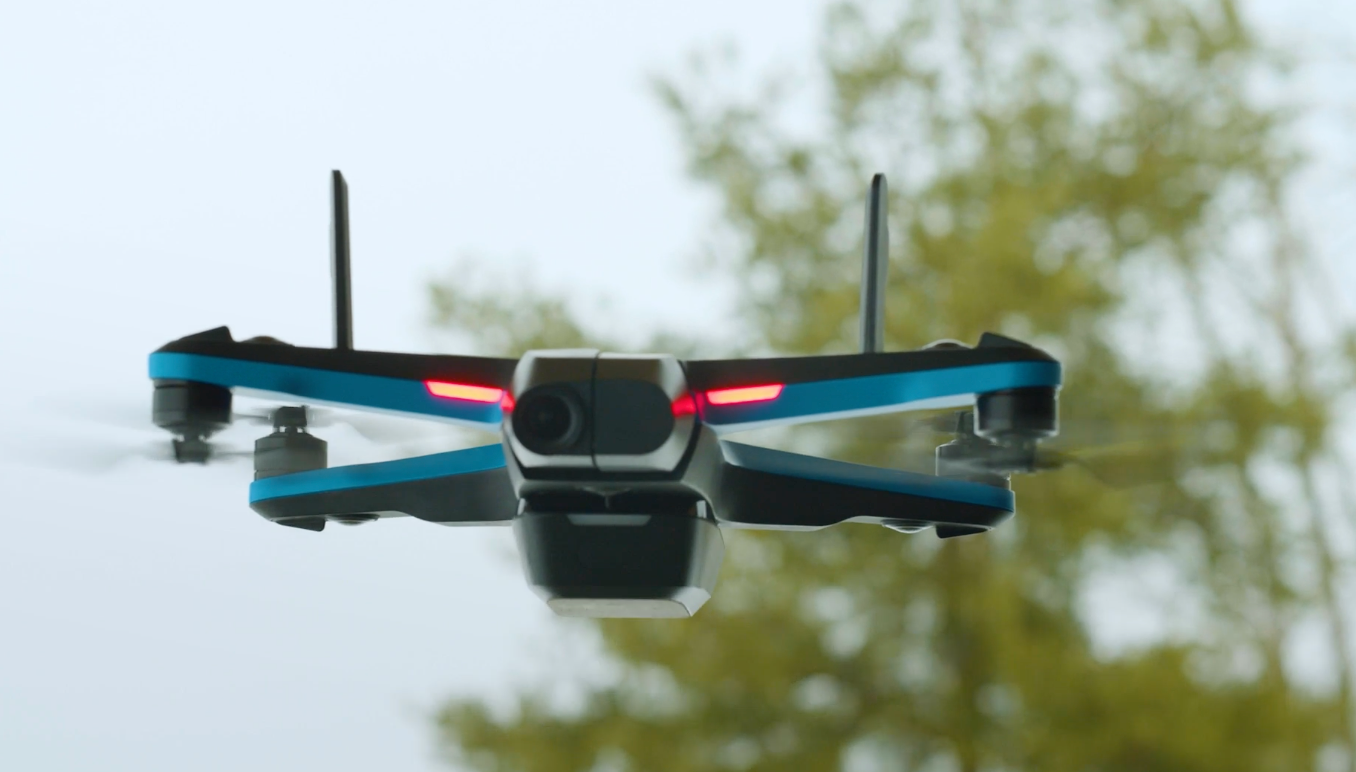
\includegraphics[width=7cm, height=5cm]{chapter2/FIGS/skydio-2.png} }}%
    \qquad
    \subfloat[\centering The DJI Matrice 600, released in 2016, is a fully-programmable autonomous drone with support for native onboard GPUs. Its huge size limits practical deployment~\cite{DJIMatrice}.]{{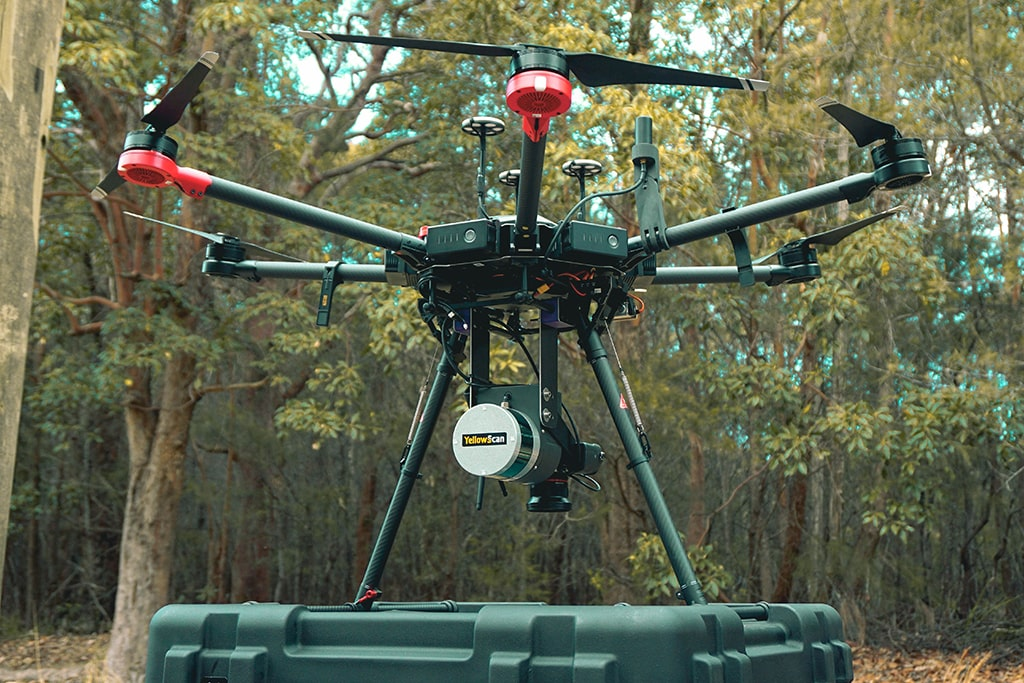
\includegraphics[width=7cm, height=5cm]{chapter2/FIGS/matrice600-2.png} }}%
    \caption{Evolution of Drone Technology}%
    \label{fig:20th-century-drones}%
\end{figure}

In the mid 2010s, drone technology started to shift away from exclusive manual piloting. The release of commercial autopilots like Pixhawk4 and Ardupilot enabled the rise of miniaturized (under 2~kg) multirotor drones which could perform limited autonomous flight such as following preset GPS waypoints~\cite{Pixhawk,Ardupilot}. Later, this was extended to semi-autonomous visual tracking and autonomous obstacle avoidance in quadrotor offerings like the DJI Phantom 4 and the Skydio 2~\cite{DJIPhantom4,Skydio2}. At the same time, growing investment in commercial fully-autonomous drones yielded the first off-the-shelf products. The DJI Matrice series (around 1~kg) was the most prominent of these, and it offered fully-autonomous capabilities using an onboard embedded computer, the DJI Manifold~\cite{DJIMatrice}.

While the drone space is diverse in both aircraft size and type, this thesis will focus on quadrotor drones. Quadrotors are by far the most common drone type and have a number of advantages over fixed-wings and helicopters. Namely, they are affordable, easy to use, and are very stable in flight. These make them perfect for tasks involving aerial imagery analysis which are the main focus of this thesis. For the rest of this document, all mention of ``drones'' will refer to quadrotor aircraft.

\begin{figure}
    \centering
    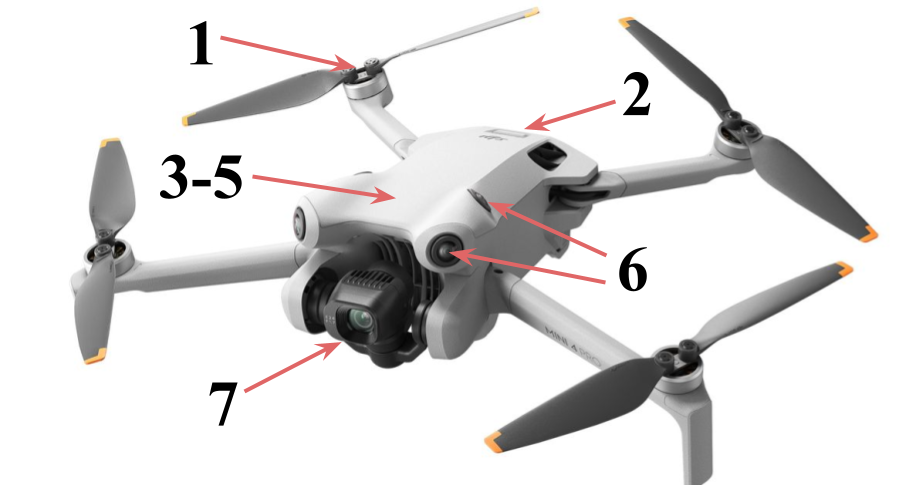
\includegraphics[width=0.75\linewidth]{chapter2/FIGS/anatomy.png}
    \begin{captext}
    \small \\ The main components of a modern consumer drone: \\\textit{\textbf{1.} rotors, \textbf{2.} hot-swappable battery, \textbf{3.} autopilot, \textbf{4.} sensor module, \\ \textbf{5.} companion computer, \textbf{6.} stereo cameras, \textbf{7.} gimbal camera.}
    \end{captext}
    \caption{Quadrotor Drone Anatomy}
    \label{fig:drone-anatomy}
\end{figure}

\subsection{Anatomy of a Drone}
Modern quadrotor drones are made up of several key components. Broadly, these accomplish one of four tasks: \textit{low-level flight control, high-level flight control, power, and sensing}. Figure~\ref{fig:drone-anatomy} uses the DJI Mini 4 Pro~\cite{DJIMini4}, a popular consumer drone, to illustrate these components:

\begin{enumerate}
    \item \textbf{Rotors} (low-level flight control): provide lift to the aircraft. Opposing pairs counter-rotate to provide stability~\cite{Allain2017}. Rotors are coordinated by the electronic speed controller (ESC), a micro-controller connected to the \textit{Autopilot} module~\cite{Nagel2023}.
    \item \textbf{Battery} (power): delivers power to all components. In many consumer drones, like the DJI Mini 4 Pro, the battery is a separate part which can be easily swapped out in the field.
    \item \textbf{Autopilot} (low-level flight control): works with the ESC to execute flight maneuvers. Uses telemetry from the \textit{Sensor Module} to compensate against the wind and maintain a stable hovering position. Acts as a software abstraction layer over all drone sensors and hardware. Also manages the radio connection to the pilot.
    \item \textbf{Sensor Module} (sensing): provides information about the drone's position and orientation, also known as telemetry. Usually made up of a GPS antenna, an inertial measurement unit (IMU)~\cite{IMU}, an altimeter, and a compass.
    \item \textbf{Companion Computer} (high-level flight control): responsible for high-level autonomous decision-making. Runs computer vision or sensor fusion algorithms then sends actuation commands to the \textit{Autopilot} based on the outputs.
    \item \textbf{Stereo Cameras} (sensing): gives a real-time depth map of the drone's surroundings~\cite{Stereo}. This enables full 360-degree obstacle avoidance. Not a feature on all consumer drones but becoming increasingly common.
    \item \textbf{Gimbal Camera} (sensing): the main camera through which the drone visually senses its surroundings. Able to pitch, yaw, or roll as commanded by the \textit{Autopilot}.
\end{enumerate}
In some cases, drones may be equipped with special equipment like LIDAR, time-of-flight sensors, RTK modules, and cellular modems. However, these are rare and are usually a feature of purpose-built aircraft for specific mission sets. 

\begin{figure}
    \centering
    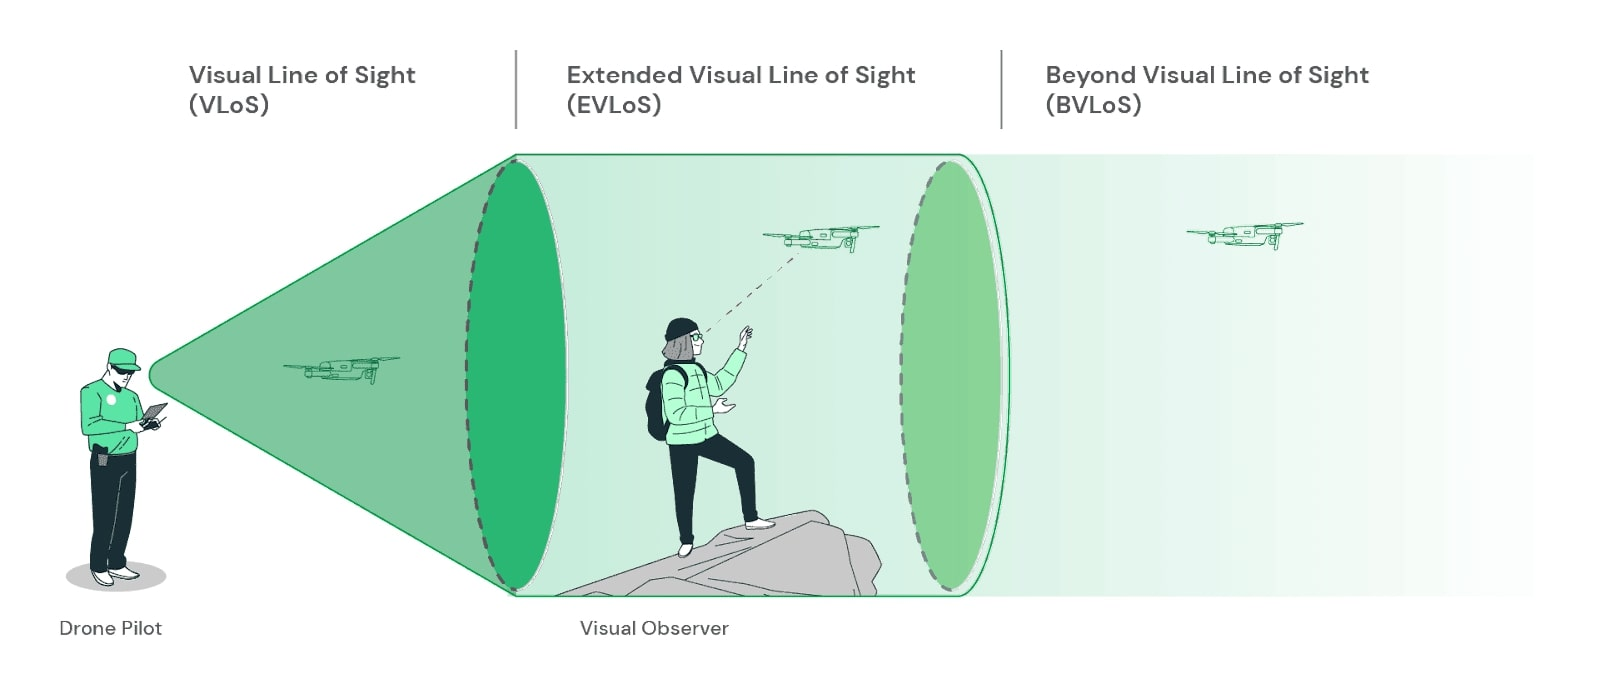
\includegraphics[width=1.0\linewidth]{chapter2/FIGS/bvlos.jpg}
    \caption{Types of Line-of-Sight Operation}
    \label{fig:bvlos}
\end{figure}

\subsection{Regulation in Civilian Airspace}
Drones like the DJI Mini 4 Pro and others are available globally for purchase, generally without the need for a license. This has led to a rapid dissemination of drones to consumers across the world and has spurred government regulators into action. This regulation serves one major purpose: to prevent potential damage to people or property due to in-flight emergencies. In the United States, the Federal Aviation Administration (FAA) introduced the Part 107 regulation in 2016~\cite{Flexairco}. This explicitly outlined the classes of UAVs allowed to fly over people, citing that only aircraft under 0.55~lbs or 250~g enjoyed near-unconditional approval~\cite{FAA2021}. In Europe, the European Union Aviation Safety Agency (EASA) has introduced similar regulation, only permitting flights over uninvolved pedestrians for drones under 250~g~\cite{EASA}. Flights over assemblies of people are not allowed for any weight class. In other countries, drones under 250~g are not regulated at all~\cite{IndiaRegulation,ChinaRegulation}.

In addition to weight regulation for flights over people, most countries also have restrictions on beyond visual line-of-sight (BVLOS) operation of heavy drones. BVLOS operation is defined as flying outside the visual range of the pilot (referred to as the RPIC, or remote pilot-in-command by the FAA) and outside the visual range of an observer within radio contact with the RPIC~\cite{BVLOS}. Figure~\ref{fig:bvlos} shows the different classes of line-of-sight operations.

\subsection{The Current Drone Market}
\label{sec:current-market}
As a result of both regulation and consumer demand, the current drone market is segmented into three loose categories: fully-autonomous, semi-autonomous, and manually piloted drones. Each of these inhabits a different weight and mission class, and are designed to operate in different regulatory environments. Table~\ref{tab:drone-apps} exhibits the main applications that drones are designed for. Generally, depending on regulation in the mission area, either a semi-autonomous (heavily-regulated) or fully-autonomous (lightly-regulated) drone will be used. 

\begin{enumerate}
    \item \textbf{Manually-Piloted Drones}: Manually-piloted drones are designed for hobbyist consumers, usually for the purpose of drone racing or recreational RC flight. They have no onboard compute, are not programmable, and must be manually piloted at all times to function. An example of a manually-piloted drone is the iFlight Cidora. This class of drone is extremely lightweight and very affordable compared to both semi- and fully-autonomous drones. The iFlight Cidora weighs 115~g and costs \$295 per unit~\cite{Cidora}. Most manually-piloted drones are so light that they avoid regulation.
    \\
    \item \textbf{Semi-Autonomous Drones}: Semi-autonomous drones have limited onboard compute and cannot perform active vision tasks without a human in the loop. They are typically equipped with a commercial autopilot like Pixhawk4 which enables autonomous following of GPS waypoints and automatic stabilization. They are not intended to operate BVLOS and often require a constant link to the RPIC (remote pilot in command). An example of a semi-autonomous drone is the Parrot Anafi. It is programmable and has no onboard compute, but can follow GPS waypoints and perform limited visual tracking by offloading to the RPIC's controller. This class of drone is lightweight and affordable compared to fully-autonomous drones, and can usually be flown in dense urban environments with minimal regulatory hurdles. The Parrot Anafi weighs 320~g and costs \$470 per unit~\cite{ParrotAnafi}.
    \\
    \item \textbf{Fully-Autonomous Drones}: Fully-autonomous drones have significant compute resources onboard and are able to analyze their own sensor streams in real time. They can perform active vision tasks without human assistance and can operate BVLOS. They also are fully-programmable, often outfitted with an onboard computer and flight control API. An example of a fully-autonomous drone is the DJI Matrice series. This class of drone is typically heavy and expensive. The Matrice 300 RTK, for instance, is over 3.5~kg and over \$10,000 per unit~\cite{Matrice300RTK}. Because of their size and weight, fully-autonomous drones are generally limited to use in rural areas away from people or property.
    \\
\end{enumerate}
In reality, most drones share traits from all three of these categories, and seldom fit into one cleanly. This motivates viewing the drone space as a ``spectrum of autonomy'', from least (manually-piloted) to most (fully-autonomous). Figure~\ref{fig:spectrum} shows the capabilities of several popular drones and where they would lie on this theoretical spectrum.


\begin{table}
    \centering
    \rowcolors{2}{gray!10}{white}
    \begin{tabularx}{\textwidth}{| m{2.8cm} | m{12.5cm} |}
        \hline
        \centering \makecell{Precision\\Agriculture} & 
        \small Drones are very useful for precision agriculture, with uses in monitoring, planting, irrigation, and pollination. They are easily scalable for large crop fields and can cover more area than ground-based solutions~\cite{Croptracker}. Most drone agriculture solutions use heavy, fully-autonomous platforms since rural areas have less strict regulation. \\[0.1cm]
        \hline
        \centering\makecell{Search and\\Rescue} & 
        \small Aerial vehicles have historically been a vital component in search and rescue. Drones fit nicely into this role, allowing search and rescue teams to scan an area at a much lower altitude than they could with traditional aircraft. They have seen real world use in the wake of the 2010 Haiti earthquake and other natural disasters~\cite{SARDrone}. \\[0.1cm]
        \hline
        \centering\makecell{Package\\Delivery} &
        \small For many years, drones have been touted as the future of last mile package delivery. This is because they can operate with higher cost-efficiency for small size items and can reach areas that are not well-connected by traditional infrastructure~\cite{PackageDrone}. Amazon has invested heavily in Prime Air, a drone-based extension to its popular Prime delivery service. However, this project has been sidelined by FAA regulation~\cite{Link2023}. Other companies like Zipline have had more success, using drones to make 1 million deliveries to remote areas~\cite{ForbesZiplineDeliveries}. \\[0.1cm]
        \hline
        \centering\makecell{Structure\\Inspection} &
        \small Recently, drones have emerged as a useful tool for structure inspection. They are able to reach inaccessible sections of structures due to their small size and maneuverability. More importantly, they are much safer and efficient than a human inspector. In 2022, the U.S. Bureau of Labor Statistics estimated that 1 in every 5 construction workplace deaths was due to falls~\cite{ConstructionFalls}. Drones allow pilots to view unsafe areas with no personal risk. This has increased the frequency of building inspection checkups, ensuring prompt, safe maintenance on failing infrastructure~\cite{InfrastructureInspection}. \\[0.1cm]
        \hline
        \centering\makecell{Aerial\\Surveys} &
        \small While aerial surveys and 3D scans have been conducted for decades, drones are a new, more cost effective tool for this task~\cite{AerialPhotography}. Their ability to provide a high resolution, bird's eye view of an area combined with their flight stability, make them ideal candidates for survey work. \\[0.1cm]
        \hline
        \centering\makecell{Police\\Work} &
        \small Drones have seen an increasing role in law enforcement. Agencies use them for general surveillance, illegal activity monitoring, crime scene investigation, and many other mission sets~\cite{PoliceDrone}. Companies like Skydio and DJI focus many offerings on this market segment. \\[0.1cm]
        \hline
        \centering\makecell{Aerial\\Reconnaissance} &
        \small Modern drones have revolutionized military aerial reconnaissance. Their small size allows them to be carried with a squad and deployed on-the-fly when necessary~\cite{StarsStripes}. The U.S. military has also invested in micro-scale platforms like the Teledyne Black Hornet that could conceivably be carried by every soldier~\cite{StarsStripes}. \\[0.1cm]
        \hline
        \centering\makecell{Suicide\\Aircraft} & 
        \small Suicide drones have been one of the most impactful new weapons in the War in Ukraine. Both Russian and Ukrainian forces have used small quadcopters like the DJI Mavic 3 to deliver bomb payloads~\cite{BBCKamikaze}. These have been very effective against slow moving targets like tanks~\cite{FPKamikaze}. Some fear that this technology could lead to a new breed of terrorist attacks~\cite{Pledger2021}. \\[0.1cm]
        \hline
        \centering\makecell{Anti-Drone\\Defense} &
        \small As the threat of drones has increased, the investment in drone defense systems has surged. Companies like Anduril have tackled this problem by using specialized drones to take down other hostile drones. Their Anvil kinetic interceptor destroys other UAVs by smashing into them at high speeds~\cite{Anvil}. \\[0.1cm]
        \hline
    \end{tabularx}
    \caption{Drone Applications}
    \label{tab:drone-apps}
\end{table}

\begin{figure}[]
    \centering
    \begin{tabular}{|c|c|c|c|c|c|}
        \hline
           \rowcolor{lightgray!50}
         \textbf{Drone} & \textbf{Autopilot} & \textbf{Avoidance} & \textbf{Tracking} & \textbf{Programmable} & \textbf{Compute} \\
         \hline
         iFlight Cidora & \cellcolor{green!20}None & \cellcolor{green!20}None & \cellcolor{green!20}None & \cellcolor{green!20}No & \cellcolor{green!20}None \\[0.1cm]
         \hline
         DJI Avata 2 & \cellcolor{orange!25}Yes & \cellcolor{yellow!20}Partial & \cellcolor{green!20}None & \cellcolor{green!20}No & \cellcolor{green!20}None \\[0.1cm]
         \hline
         Parrot Anafi & \cellcolor{orange!25}Yes & \cellcolor{green!20}None & \cellcolor{yellow!20}Assisted & \cellcolor{red!20}Yes & \cellcolor{green!20}None \\[0.1cm]
         \hline
         Skydio 2 & \cellcolor{orange!25}Yes & \cellcolor{orange!25}Yes & \cellcolor{yellow!20}Assisted & \cellcolor{yellow!20}Partially & \cellcolor{green!20}None \\[0.1cm]
         \hline
         DJI Mini 4 Pro & \cellcolor{orange!25}Yes & \cellcolor{orange!25}Yes & \cellcolor{yellow!20}Assisted & \cellcolor{yellow!20}Partially & \cellcolor{green!20}None \\[0.1cm]
         \hline
         Skydio 2 & \cellcolor{orange!25}Yes & \cellcolor{orange!25}Yes & \cellcolor{red!20}Yes & \cellcolor{yellow!20}Partially & \cellcolor{red!20}Yes \\[0.1cm]
         \hline
         DJI Matrice 300 RTK & \cellcolor{orange!25}Yes & \cellcolor{orange!25}Yes & \cellcolor{red!20}Yes & \cellcolor{red!20}Yes & \cellcolor{red!20}Yes \\[0.1cm]
         \hline
    \end{tabular}
    \\[0.2cm]
    \begin{captext}
        \small Capabilities are colored according to whether they are typically associated with manually-piloted (green), semi-autonomous (yellow), both semi- and fully-autonomous (orange),  or fully-autonomous (red) drones. Assisted tracking means that a human pilot must help the drone in order for it to function properly.
    \end{captext}
    \centering
    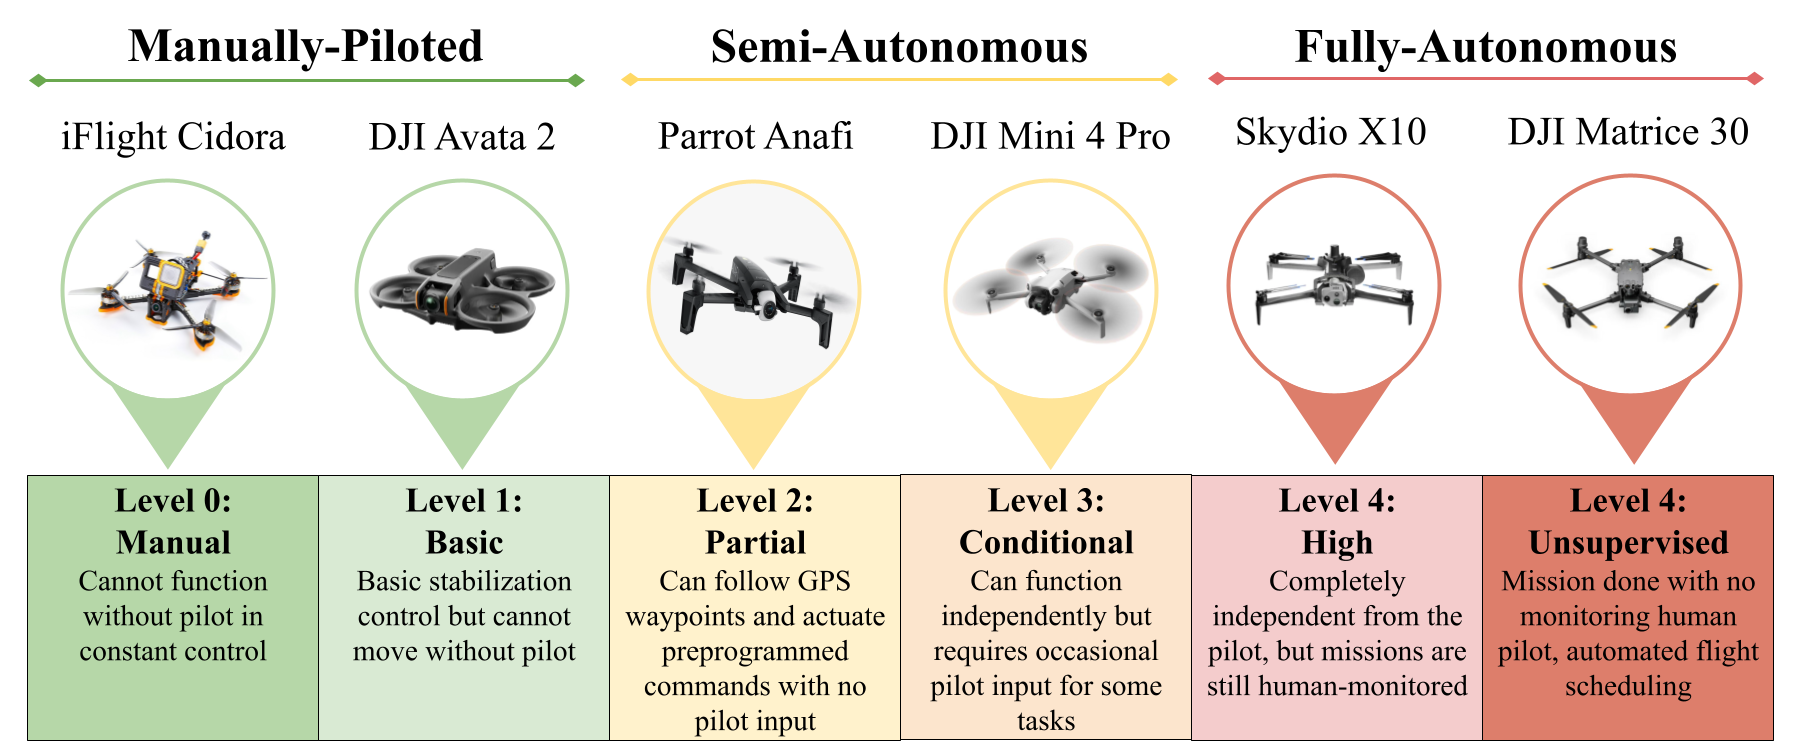
\includegraphics[width=1.0\linewidth]{chapter2/FIGS/spectrum.png}
    \begin{captext}
        \small Based on the capability set of each drone, I have roughly placed them on the theoretical spectrum of autonomy. This is an entirely subjective categorization. Others may differ on how to define each category and which drones belong in them.
    \end{captext}
    \caption{The ``Spectrum of Autonomy''}
    \label{fig:spectrum}
\end{figure}

\subsection{What is Holding Drones Back?}
\label{sec:problems}
As presented by Table~\ref{tab:drone-apps}, there are many applications where drones have been useful. However, it is my belief that they still have not lived up to their true potential. Many of the listed tasks, such as aerial surveys, building inspection, and police surveillance, are still done using full manual or human-assisted control in densely populated areas. Yet, many if not all of these tasks could benefit greatly from full-autonomy, especially in or around cities. Surveys or inspection flights could be performed daily, without human supervision, with an auto-generated report sent out for engineers to look over. This could greatly reduce costs and prevent critical infrastructure failures, potentially saving lives~\cite{Dorafshan2018}. Automated police surveillance could free up officers, reduce training overhead, and provide round-the-clock monitoring without any risk of fatigue. So why have fully-autonomous platforms failed to see widespread use in these urban applications, when they have been used with great success elsewhere?

The answer is complicated, but I believe that there are five clear problems facing fully-autonomous drones in dense urban settings: \\[0.1]
\begin{enumerate}
    \item \textbf{Weight}: fully-autonomous aircraft are heavy, as discussed in Section~\ref{sec:current-market}. This is because they require onboard compute like GPUs to operate which drive up weight. This directly clashes with most international drone regulation which becomes progressively more restrictive over 250~g. \\[0.1]
    \item \textbf{Usability}: the majority drone users have limited or non-existent programming experience. Unfortunately, most commercial fully-autonomous offerings today demand skilled programmers to operate efficiently and safely. This makes it daunting for inexperienced users to adopt a fully-autonomous platform. \\[0.1]
    \item \textbf{Versatility}: there is a major trade-off in current fully-autonomous drone products between weight and versatility. Heavy platforms which carry generalized compute hardware like CPUs and GPUs are versatile since they can run most kinds of software natively. On the other hand, lightweight platforms cannot carry generalized compute due to weight constraints, and thus usually carry specialized compute for only one or two mission types. \\[0.1]
    \item \textbf{Portability}: drone manufacturers have their own, tightly integrated software stack that does not work with other drone models. This all or nothing approach means that a consumer must stick within the hardware ecosystem or be forced to buy an entirely new fleet of drones. \\[0.1]
    \item \textbf{Cost}: fully-autonomous drones typically cost around ten times the cost of comparable semi-autonomous drones. This makes them much less economical to deploy at scale. 
    \\[0.1]
\end{enumerate}
At the time of writing this thesis, no commercial product has addressed all five of these concerns.


\section{Prior Research}
\label{sec:prior-work}
In parallel to commercial efforts, autonomous drone research has surged in recent years. Real-time execution of active vision tasks has been a key driver. Schedl et al proposed an autonomous drone design for classification-driven adaptive search and rescue in densely forested environments~\cite{Schedl2021}. George et al demonstrated a drone inspection system which could localize the drone's camera view onto a 3D model of a target structure in real time~\cite{George2019}. Chen et al showed an efficient drone onboard computation model for visual object tracking~\cite{Chen2018}. Many other projects have explored similar applications in surveillance, wildlife monitoring, racing, and obstacle avoidance~\cite{Apvrille2014,Li2020,Devos2018,Alsalam2017,Ward2016}.  

A growing number of researchers have identified some of the problems outlined in Section~\ref{sec:problems} (\textit{weight}, \textit{usability}, \textit{versatility}, \textit{portability}, and \textit{cost}) as important research areas. In this section, I will present projects that attempt to solve these problems. I will also discuss their limitations and why their solutions have not fully addressed the issues I outlined.

\subsection{Weight}
Since as early as 2009, the drone research community has recognized the importance of lightweight aircraft in real world applications~\cite{Burkle2011, Burkle2009}. Lightweight ($\leq 450$~g) autonomous drones have many benefits over their heavier counterparts: they are safer to operate, have simpler transportation logistics, and have a lower noise profile. It was theorized that achieving such lightweight autonomy would enable the vision of cooperative drone swarms~\cite{Floreano2015}. Since the mid 2010s, much work has focused on bringing high-level autonomy to small, lightweight drones. Schmid et al proposed a sub-1~kg aircraft design which could perform unassisted visual navigation~\cite{Schmid2014}. Palossi et al developed visual navigation and human pose estimation software which runs onboard 27~g drones~\cite{Palossi2019,Palossi2021}. M{\"u}ller et al demonstrated a depth-based obstacle avoidance system for 35~g drones~\cite{Muller2023}. Many of these projects suffer from similar issues of \textit{portability}. That is, they either use purpose-built aircraft or function on one type of aircraft. There is little ability to deploy these systems to different drone hardware, a serious drawback in an ever-changing drone landscape. 

\subsection{Usability}
\label{sec:development-platforms}
For many years, drone research did not consider usability. Many projects used custom-built aircraft with no guidance on how to replicate the platform for other researchers. Others provided autonomous software which was only usable by experts, and thus could not be leveraged by average developers. These days, the drone research community has started to recognize the importance of usability. Beseda et al presented a mission-oriented control infrastructure for easily managing swarms of autonomous UAVs~\cite{Besada2019}. Mottola et al proposed a simple but expressive API for drone team control~\cite{Mottola2014}. Tilley et al developed a block programming language that could allow children to program autonomous drones~\cite{Tilley2017}. While this work is useful, these projects do not present a practical integration strategy with real consumer drones. There is no consideration of \textit{portability} or \textit{weight}, both very important for public deployment.

\subsection{Versatility}
Mission versatility is a feature that most heavy fully-autonomous drones already possess, since they carry generalized compute like CPUs and GPUs which can run GPLs (general-purpose programming languages) and inference deep neural networks with relatively low latency. However, achieving this versatility on lightweight drones is an enduring challenge. This is because miniaturizing generalized compute hardware is difficult, and weight-optimized compute hardware is inflexible~\cite{Hu2022}. Still, many have tried to modify lightweight onboard hardware to be able to run heavyweight computer vision. Albanese et al propose a neural accelerator modification to a Raspberry Pi which could be flown onboard small UAVs~\cite{Albanese2022}. Zhang et al demonstrate an FPGA architecture for drones that can inference neural networks with much lower power demand than GPUs~\cite{Zhang2022}.

\begin{figure}
    \centering
    \subfloat[\centering Bitcraze Crazyflie\\(27~g)]
    {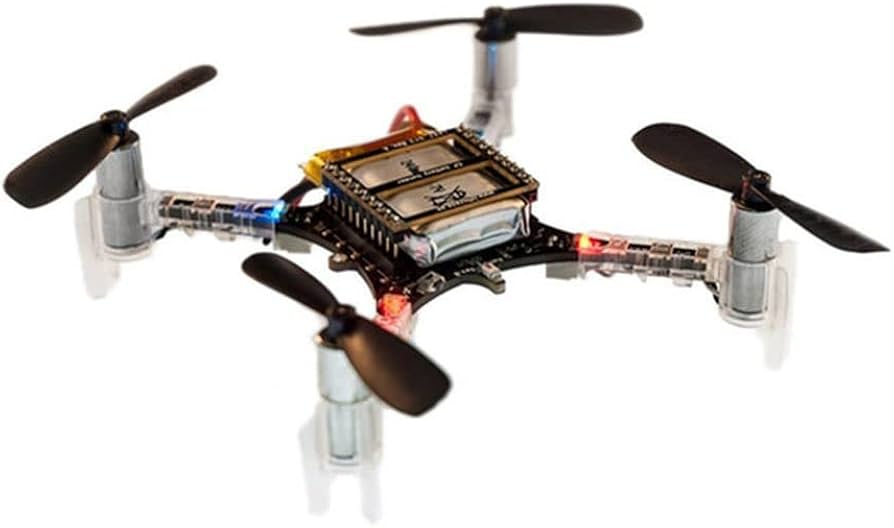
\includegraphics[width=0.30\textwidth, height=1.5in]{chapter2/FIGS/crazyflie.jpg}}
    \qquad
    \subfloat[\centering Modal AI Starling\\(280~g)]
    {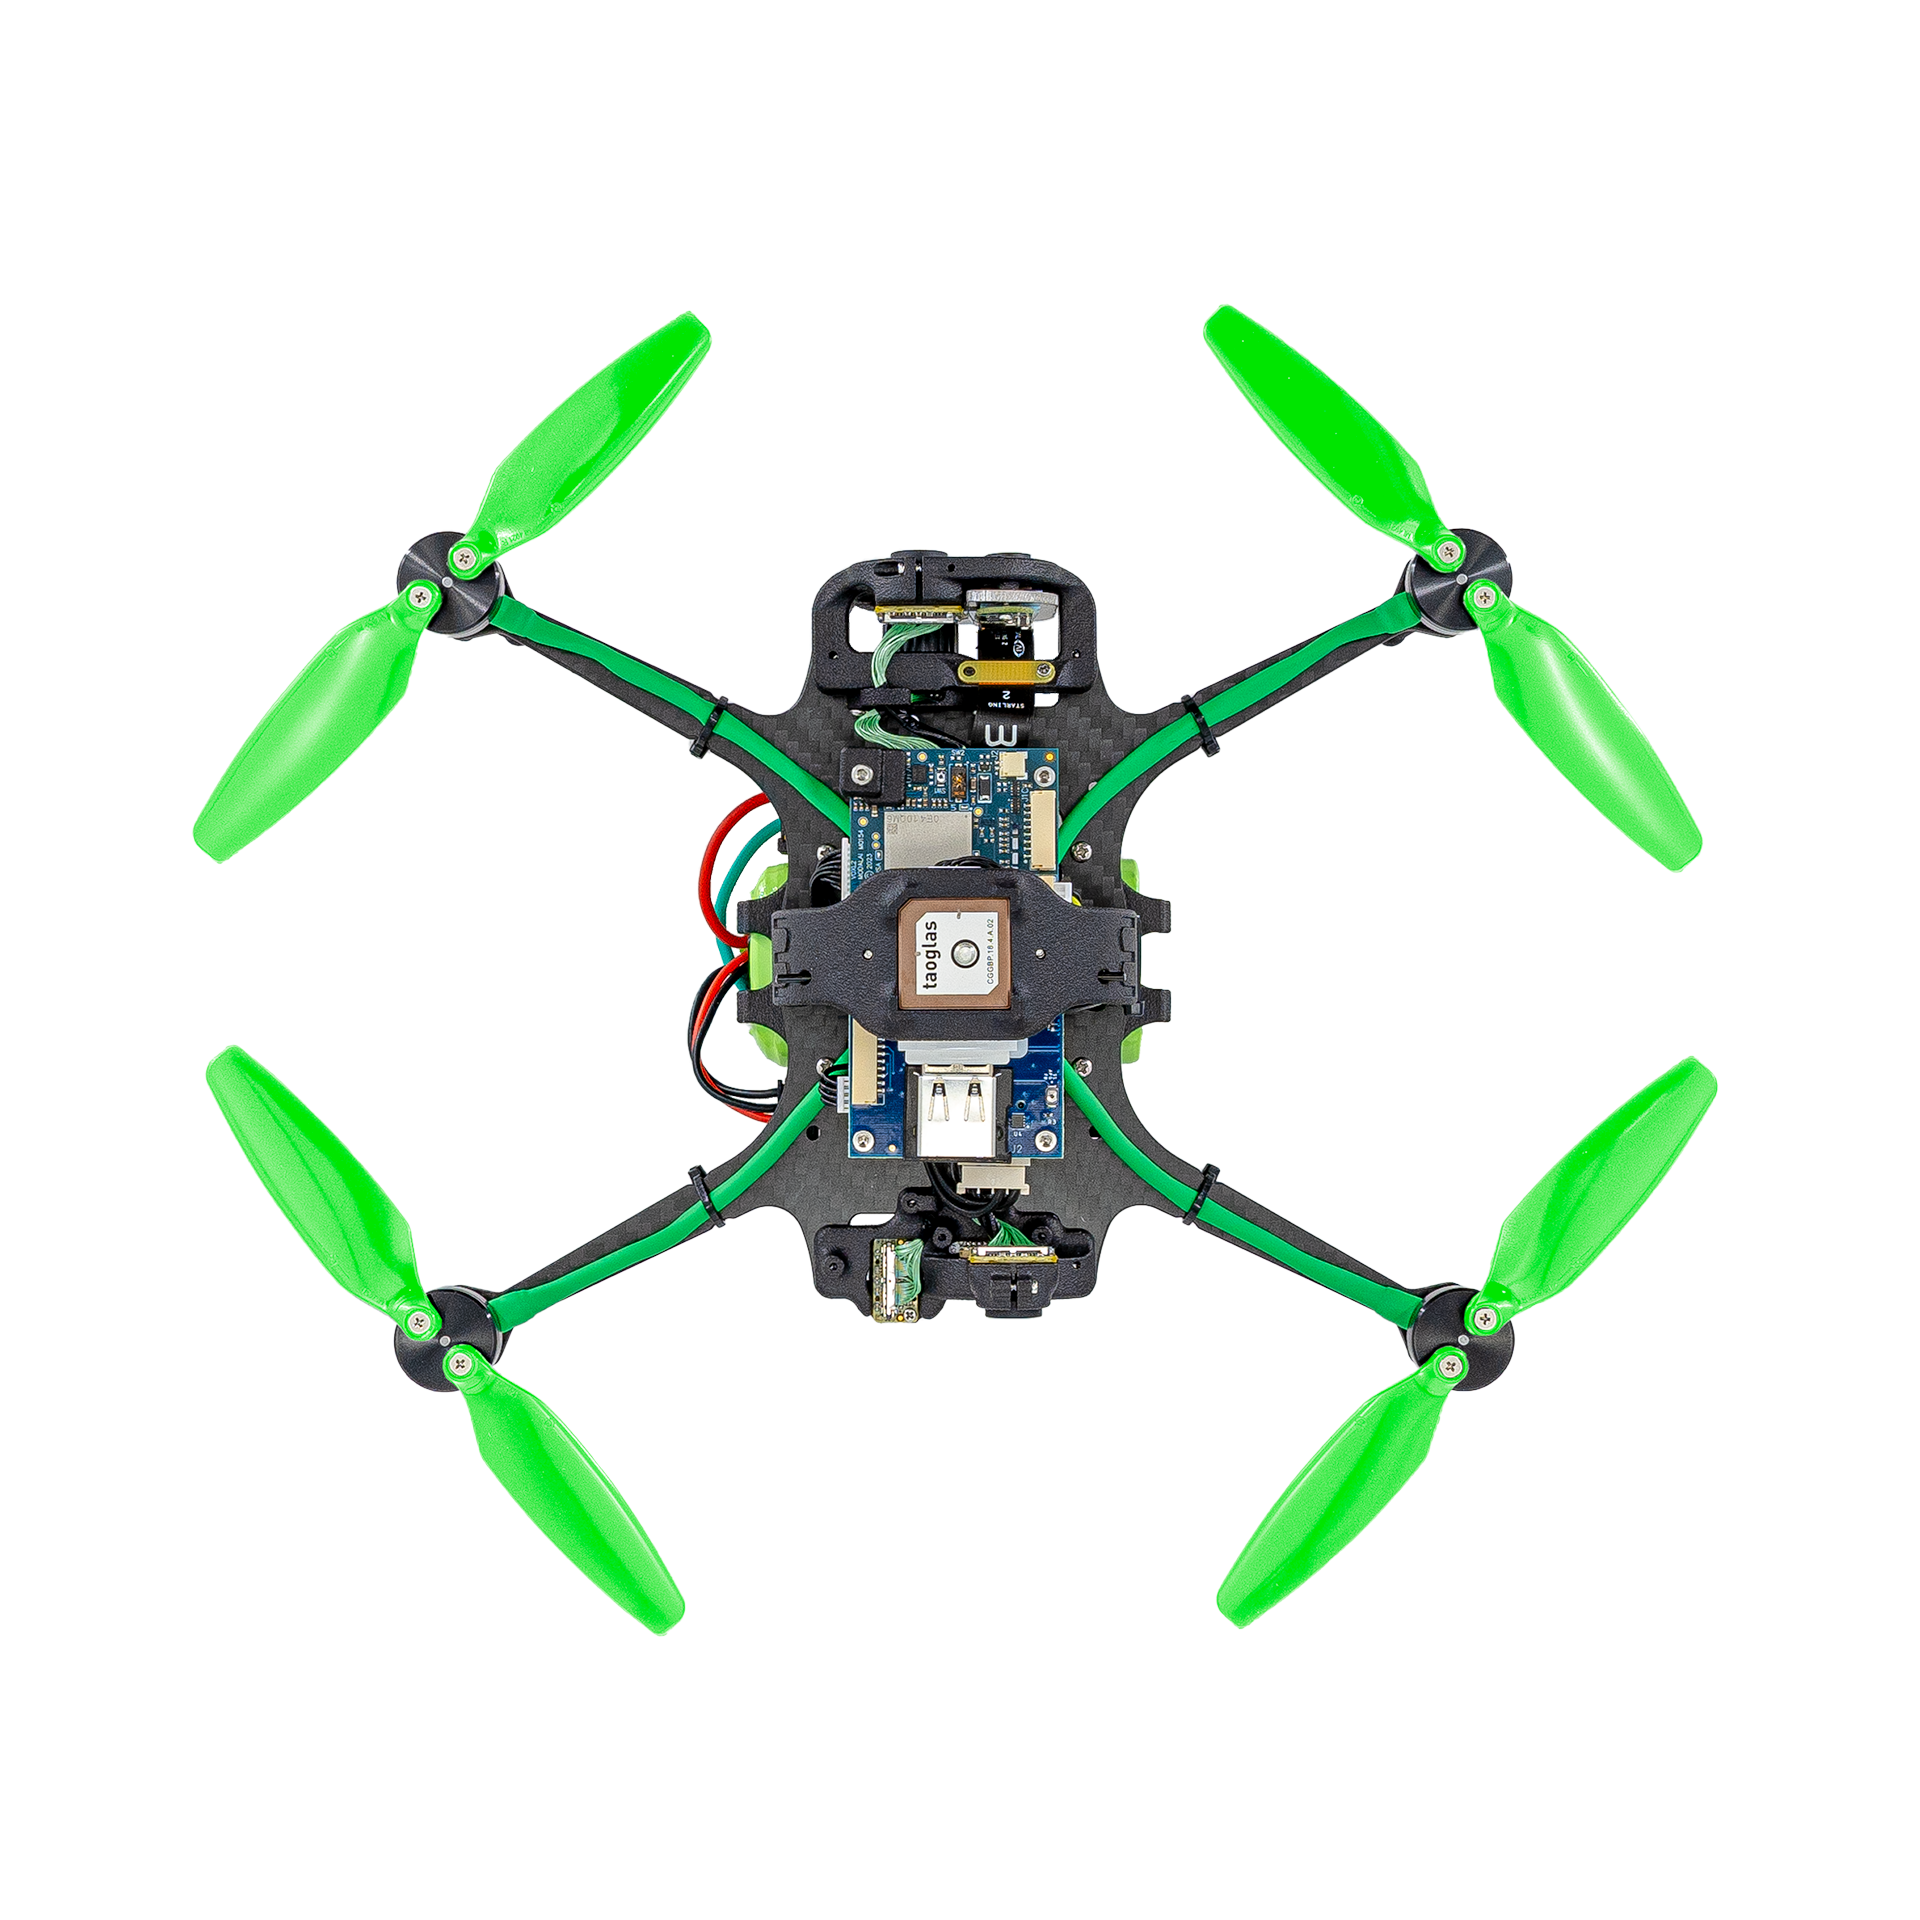
\includegraphics[width=0.30\textwidth, height=1.75in]{chapter2/FIGS/starling-2.png}}
    \caption{Consumer Drone Development Platforms}
    \label{fig:drone-dev-platforms}
\end{figure}

\subsection{Portability}

\subsection{Cost}

\section{A Key Insight: the Onboard Compute Trade-off}
\label{sec:better-autonomous-drones}
The key factors of \textit{weight}, \textit{usability}, \textit{versatility}, \textit{portability}, and \textit{cost} all hinder autonomous drone development and deployment, yet no proposed system has solved all of these issues simultaneously. Central to this problem is the trade-off between heavy, generalized, onboard compute that supports common programming ecosystems but exceeds regulatory limits, and lightweight, specialized, onboard compute that can only run tailor-made programs, but is light enough to fly within regulatory bounds. 





\chapter{Connecting COTS Drones to the Edge}
%\appendix
%\include{appendix}

\backmatter

%\renewcommand{\baselinestretch}{1.0}\normalsize

% By default \bibsection is \chapter*, but we really want this to show
% up in the table of contents and pdf bookmarks.
\renewcommand{\bibsection}{\chapter{\bibname}}
%\newcommand{\bibpreamble}{This text goes between the ``Bibliography''
%  header and the actual list of references}
\bibliographystyle{plainnat}
\bibliography{thesis} %your bib file

\end{document}